%!TEX root=masterproef.tex
\chapter{Besluit}
\label{besluit}

\chapterprecishere{
At least for the people who send me mail about a new language that they're
designing, the general advice is: do it to learn about how to write a compiler.
Don't have any expectations that anyone will use it, unless you hook up with
some sort of organization in a position to push it hard. It's a lottery, and
some can buy a lot of the tickets. There are plenty of beautiful languages
(more beautiful than C) that didn't catch on. But someone does win the lottery,
and doing a language at least teaches you something.
\par\raggedleft--- \textup{Dennis Ritchie (1941-2011)},\\
Creator of the C programming language and of UNIX}

In dit besluit belichten we het voorstel van deze masterproef vanuit
verschillende invalshoeken. We doen dit aan de hand van een korte SWOT-analyse.

\section{Sterke punten}
\label{section:strenghts}

FOO-lang en de codegenerator slagen er in te scoren op elk van de gestelde
criteria en beantwoorden elk aspect van de probleemstelling (zie sectie
\ref{section:problem-definition}) positief: het detecteren van inbraken wordt
mogelijk gemaakt zonder eisen te stellen aan hard- en/of software. De formele
beschrijving van algoritmen vormt de basis voor een volledig geautomatiseerd
generatie- en ontwikkelingsproces, waardoor het economisch verantwoord is om
een IDS toe te voegen aan een WSN en het zelfs mogelijk is om in te spelen op
veranderende omstandigheden.

In tegenstelling tot een klassiek raamwerk, zoals bv. Di-Sec in sectie
\ref{subsubsection:di-sec}, dringt de oplossing geen specifiek raamwerk op,
maar is het zelfs in staat om met elk bestaand raamwerk samen te werken.

\section{Zwakke kanten}
\label{section:weaknesses}

Daartegenover staat wel het bouwen van de nodige modules om andere platformen
en talen te ondersteunen. Ook al is dit veelal een eenmalige kost, de
complexiteit hiervan mag niet onderschat worden.

\section{Opportuniteiten}
\label{section:opportunities}

De beperkingen die opgelegd werden aan het prototype vormen dan weer vele
opportuniteiten voor verder onderzoek en verbeteringen: het optimaliseren van
FOO-lib en de gegenereerde code op zich kan leiden tot een nog lagere impact op
\mcu en draadloze radio. Nog verdere \emph{inlining} van code of het opnemen
van FOO-lib in het generatieproces kan verstrekkende gevolgen hebben.

De mogelijkheden tot verdere analyse en simulatie, een centrale locatie voor
detectiealgoritmen en het samenbrengen van een gemeenschap hierrond, zijn
stappen die het onderzoek vooruit zouden kunnen stuwen.

\vspace{-2mm}

\section{Bedreigingen}
\label{section:threaths}

Aan het andere eind van dit spectrum blijft het feit dat er geen absolute
beveiliging kan gebouwd worden als een zwaard van Damocles boven draadloze
sensoren hangen.

Een nieuwe taal voorstellen is op zich al geen sinecure. Ze wordt immers
vrijwillig geaccepteerd, zelden opgedrongen. Zonder de onderbouw van FOO-lang
verliest de oplossing veel draagkracht.

\vspace{-2mm}

\section{De slotsom}
\label{section:bottom-line}

Deze masterproef toont aan dat codegeneratie een nuttige oplossing kan zijn
voor het implementeren van een IDS voor een WSN en kan helpen om meer te
detecteren en zo ook de informatie die we deze netwerken toevertrouwen beter te
verdedigen. Maar we mogen \'e\'en belangrijk aspect niet uit het oog verliezen:
hoeveel verdedigingslinies we ook opwerpen, hoe ingenieus onze
detectiealgoritmen ook zijn, er blijft steeds \'e\'en grote, onvoorspelbare
factor in het hele verhaal, en dat is de menselijke capaciteit om fouten te
maken.

\begin{figure}[ht]
  \centering
  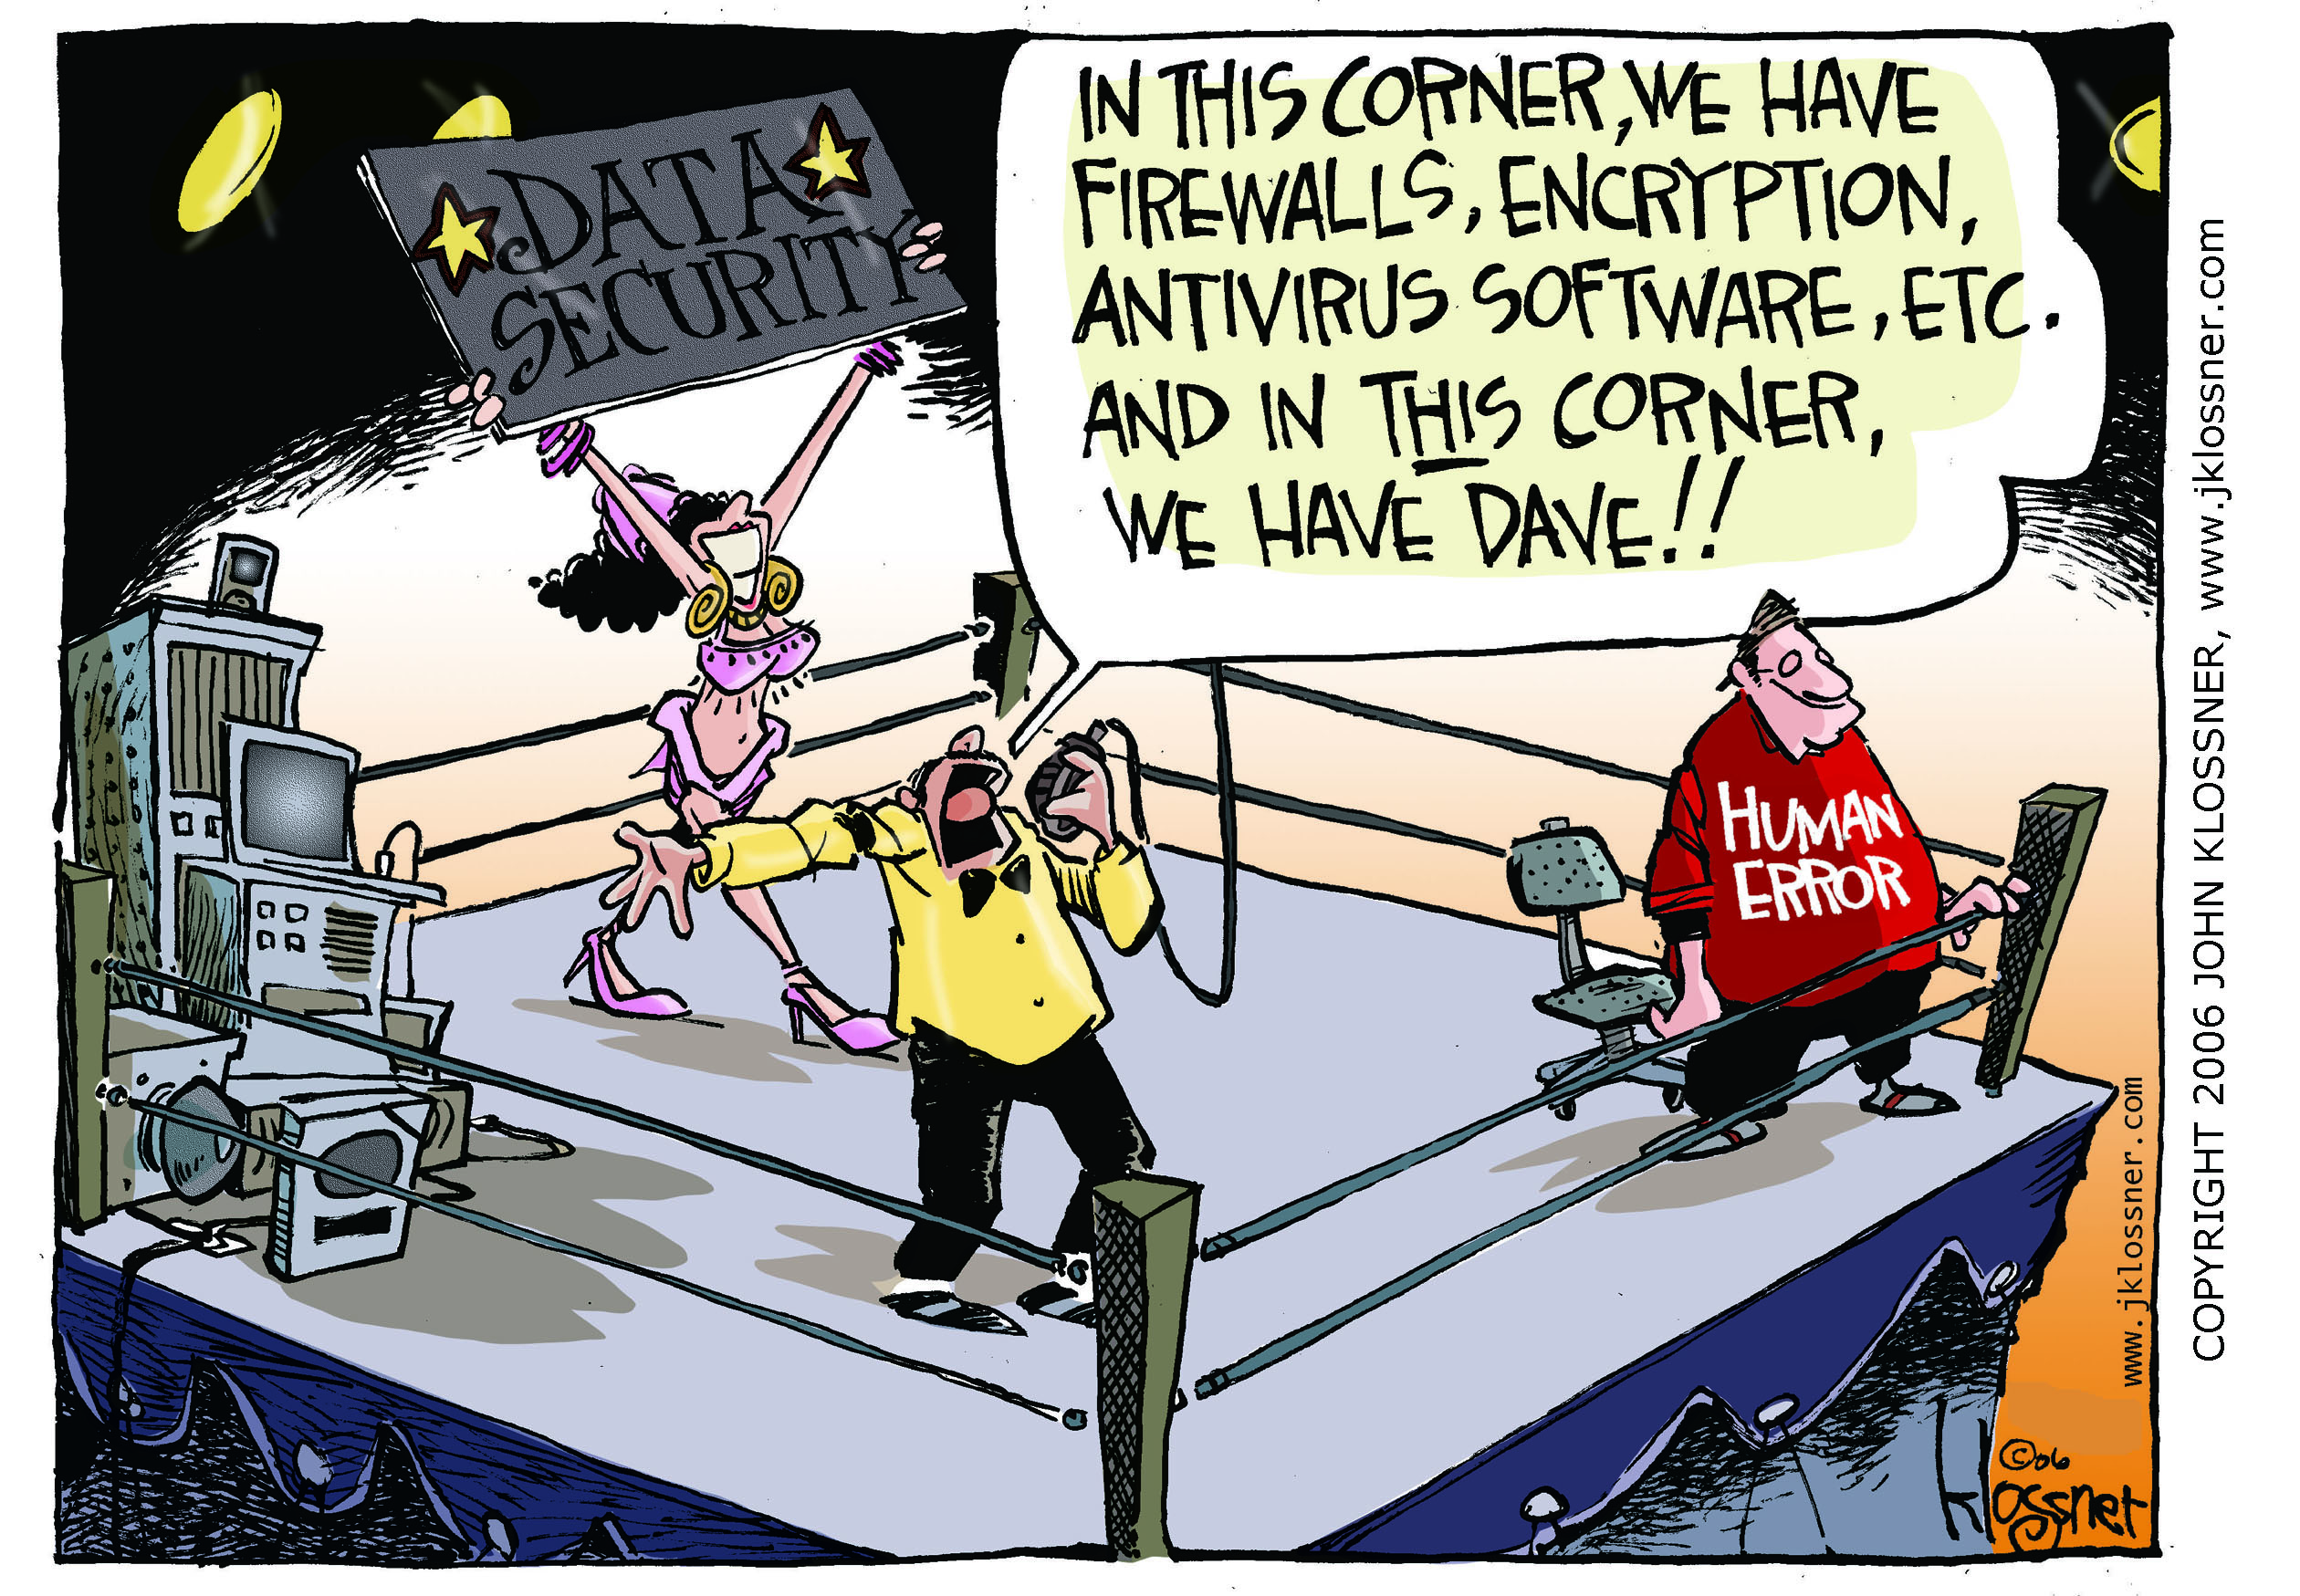
\includegraphics[width=0.72\linewidth]{resources/cartoon_human_error.jpg}
  \caption[``Human Error'']{``Human Error'' - met dank aan John Klossner}
\end{figure}
